\documentclass{article}
\usepackage{spconf}
\raggedbottom

% ==============================================================================
% PACKAGES
% ==============================================================================
\usepackage[utf8]{inputenc}
\usepackage{vntex} % Hỗ trợ tiếng Việt
\usepackage{cite}
\usepackage{amsmath,amssymb,amsfonts}
\usepackage{algorithmic}
\usepackage{graphicx}
\usepackage{textcomp}
\usepackage{xcolor}
\usepackage{booktabs}
\usepackage{algorithm}
\usepackage{caption}
\usepackage{subcaption}
\usepackage{hyperref}
\usepackage{multirow}
\usepackage{adjustbox}

% --- VIETNAMIZATION & FONT FIX ---
\makeatletter
\def\section{\@startsection {section}{1}{\z@}{-3.5ex plus -1ex minus -.2ex}{2.3ex plus .2ex}{\Large\bfseries}}
\def\subsection{\@startsection{subsection}{2}{\z@}{-3.25ex plus -1ex minus -.2ex}{1.5ex plus .2ex}{\large\bfseries}}
\def\abstract{\begin{center}{\bfseries TÓM TẮT\vspace{-.5em}\vspace{0pt}}\end{center}}
\def\keywords{\vspace{.5em}{\bfseries Từ khóa---}}
\makeatother
\renewcommand{\figurename}{Hình}
\renewcommand{\tablename}{Bảng}
\makeatletter
\@ifpackageloaded{algorithm}{\floatname{algorithm}{Thuật toán}}{}
\makeatother

\def\BibTeX{{\rm B\kern-.05em{\sc i\kern-.025em b}\kern-.08em
    T\kern-.1667em\lower.7ex\hbox{E}\kern-.125emX}}

% ==============================================================================
% DOCUMENT BEGIN
% ==============================================================================
\begin{document}

\title{BFSPMiner-Improved: Khai phá mẫu tuần tự trên luồng dữ liệu với độ dài thích ứng và khoảng trống}

\name{Thân Thị Hằng, Lê Thị Kiều Trang, Hà Tuấn Hiếu}
\address{Học viện Kỹ thuật Quân sự\\Viện Công nghệ Thông tin \& Truyền thông}

\maketitle

% ==============================================================================
% ABSTRACT
% ==============================================================================
\begin{abstract}
Khai phá mẫu tuần tự trên luồng dữ liệu là nhiệm vụ quan trọng trong khai phá dữ liệu, cho phép phân tích thời gian thực trong nhiều lĩnh vực như giám sát IoT và phân tích hành vi người dùng. Các thuật toán truyền thống thường dựa trên xử lý theo lô (batch), gây ra độ trễ cao và tiêu thụ bộ nhớ lớn, không phù hợp với luồng dữ liệu liên tục, tốc độ cao. Trong bài báo này, chúng tôi đề xuất BFSPMiner-Improved, một thuật toán khai phá mẫu tuần tự không theo lô (batch-free) được cải tiến cho môi trường thời gian thực. Phương pháp của chúng tôi giới thiệu hai cơ chế mới: (i) cơ chế Adaptive \textit{maxPatternLength} tự động điều chỉnh độ dài mẫu tối đa dựa trên entropy và áp lực bộ nhớ, và (ii) mở rộng Gap-Aware Episode Mining cho phép phát hiện các phụ thuộc thời gian linh hoạt. Thực nghiệm toàn diện trên tập dữ liệu thực tế REDD (458K sự kiện, IoT) và MSNBC (424K sự kiện, clickstream entropy cao) cho thấy: BFSPMiner-Improved tăng 84--93\% số mẫu phổ biến trên REDD và 90--188\% trên MSNBC; đạt Precision@3 lên 99,45\% (REDD) và 51,89\% (MSNBC, vượt Majority Baseline); giảm 17 lần bộ nhớ nhờ cơ chế thích ứng; và duy trì khả năng mở rộng tuyến tính với tốc độ xử lý $\sim$7.100 sự kiện/giây.
\end{abstract}

\begin{keywords}
Luồng dữ liệu, Khai phá mẫu tuần tự, Khai phá tập sự kiện, Xử lý thời gian thực, Phân tích dự đoán
\end{keywords}

% ==============================================================================
% 1. INTRODUCTION
% ==============================================================================
\section{Giới thiệu}
\label{sec:intro}

Khai phá mẫu tuần tự (sequential pattern mining -- SPM) trên luồng dữ liệu liên tục đóng vai trò ngày càng quan trọng trong nhiều ứng dụng thực tế: từ giám sát năng lượng trong hệ thống nhà thông minh, phân tích chuỗi tương tác IoT, khai thác hành vi duyệt web (clickstream), đến phát hiện bất thường trong hệ thống công nghiệp. Khác với cơ sở dữ liệu tĩnh truyền thống, luồng dữ liệu mang ba đặc trưng thách thức: (i) vô hạn và liên tục, (ii) đến với tốc độ cao, và (iii) phân bố thay đổi theo thời gian. Những đặc trưng này đòi hỏi thuật toán phải xử lý từng sự kiện theo chế độ một lượt (single-pass) trong khi kiểm soát chặt chẽ bộ nhớ.

Hầu hết các thuật toán SPM trên luồng dữ liệu hiện có đều dựa trên mô hình xử lý theo lô (batch-based), chia luồng vô hạn thành các khối cố định rồi khai phá tuần tự từng khối. Thiết kế này gây ra hai vấn đề nghiêm trọng: (1) các chuỗi mẫu nằm xuyên suốt ranh giới nhiều batch bị mất hoàn toàn, và (2) quyết định cắt tỉa cục bộ trong từng batch có thể loại bỏ các pattern có tần suất cao trên toàn cục nhưng xuất hiện rải rác. BFSPMiner~\cite{hassani2019} đã khắc phục những nhược điểm trên bằng khung khai phá batch-free sử dụng cây đảo ngược $T_0$ (inverted trie), cho phép cập nhật liên tục mà không cần chia lô. Tuy nhiên, thuật toán vẫn tồn tại hai hạn chế quan trọng được chính tác giả thừa nhận:

\begin{itemize}
    \item \textbf{Chiều dài cố định:} Tham số \texttt{maxPatternLength} cố định ($L_{max}$) buộc người dùng phải chọn trước --- giá trị quá nhỏ bỏ sót các mẫu dài có ý nghĩa, giá trị quá lớn gây bùng nổ bộ nhớ bậc hai trên luồng entropy cao.
    \item \textbf{Ràng buộc liên tiếp nghiêm ngặt:} Chỉ hỗ trợ mẫu consecutive (các sự kiện kề nhau), bỏ qua các phụ thuộc thời gian không liên tiếp --- dạng phụ thuộc phổ biến trong hành vi người dùng thực tế khi bị xen kẽ bởi các tác vụ phụ.
\end{itemize}

Để khắc phục những hạn chế này, bài báo đề xuất \textbf{BFSPMiner-Improved} với hai cơ chế cải tiến:
\begin{itemize}
    \item \textbf{Adaptive maxPatternLength:} Tự động điều chỉnh $L_{max}$ dựa trên entropy luồng và áp lực bộ nhớ, cho phép khai phá mẫu dài khi tài nguyên cho phép và thu hẹp khi cần thiết.
    \item \textbf{Gap-Aware Episode Mining:} Mở rộng quá trình sinh mẫu để chấp nhận tối đa $g$ sự kiện xen giữa, nắm bắt các phụ thuộc hành vi không liên tiếp.
\end{itemize}

Thực nghiệm toàn diện trên hai tập dữ liệu thực tế --- REDD (458K sự kiện IoT, entropy thấp) và MSNBC (424K sự kiện clickstream, entropy cao) --- xác nhận giả thuyết trên. Trên MSNBC, BFSPMiner-Base (thuật toán gốc) chỉ đạt Precision@3 là 25,65\%, \textit{thấp hơn cả} chiến lược Naive-Majority (49,53\%), trong khi BFSPMiner-Improved đạt \textbf{51,89\%}. Trên cả hai tập dữ liệu, số lượng mẫu phổ biến tăng nhất quán \textbf{84--188\%}.

Các đóng góp chính của công trình bao gồm:
\begin{itemize}
    \item[(i)] Đề xuất cơ chế Adaptive \textit{maxPatternLength} dựa trên entropy và áp lực bộ nhớ, giảm tới 17 lần bộ nhớ so với cấu hình chiều dài cố định trên luồng entropy cao.
    \item[(ii)] Mở rộng Gap-Aware Episode Mining cho khung batch-free, tăng 84--188\% số mẫu phổ biến và gần gấp đôi Precision@3 trên MSNBC (25,76\% $\rightarrow$ 47,47\% chỉ với $g = 2$).
    \item[(iii)] Đánh giá thực nghiệm nghiêm ngặt trên hai tập dữ liệu đại diện cho hai lớp bài toán (IoT entropy thấp và clickstream entropy cao), bao gồm so sánh với bốn baseline (Naive-Random, Naive-Majority, BFSPMiner-Base, BFSPMiner-Improved) và nghiên cứu cắt bỏ (ablation study) cho từng thành phần.
    \item[(iv)] Triển khai Python ổn định với mã nguồn mở\footnote{\url{https://github.com/hangthan/bfspminer-improved}} và pipeline thực nghiệm có khả năng tái tạo cao.
\end{itemize}

Phần còn lại của bài báo được tổ chức như sau. Phần~\ref{sec:related} trình bày các công trình liên quan. Phần~\ref{sec:preliminaries} giới thiệu các khái niệm cơ bản và định nghĩa bài toán. Phần~\ref{sec:proposed} mô tả chi tiết phương pháp đề xuất. Phần~\ref{sec:experiments} trình bày đánh giá thực nghiệm. Phần~\ref{sec:discussion} thảo luận kết quả. Cuối cùng, Phần~\ref{sec:conclusion} kết luận và đề xuất hướng phát triển.

% ==============================================================================
% 2. RELATED WORK
% ==============================================================================
\section{Các nghiên cứu liên quan}
\label{sec:related}

\textbf{Khai phá mẫu tuần tự trên dữ liệu tĩnh.} Khai phá mẫu tuần tự (SPM) được giới thiệu lần đầu bởi Agrawal và Srikant~\cite{agrawal1995}, nhằm phát hiện các chuỗi con xuất hiện thường xuyên trong cơ sở dữ liệu chuỗi. Srikant và Agrawal~\cite{srikant1996} sau đó mở rộng với GSP, hỗ trợ ràng buộc gap và window. Hai hướng tiếp cận chính đã phát triển: SPADE~\cite{zaki2001} sử dụng biểu diễn dọc (vertical format) với phép nối id-list, trong khi PrefixSpan~\cite{pei2001} khai thác theo chiếu prefix (prefix-projected growth), tránh hoàn toàn việc sinh ứng cử viên. Yan et al.~\cite{yan2003} đề xuất CloSpan để khai phá hiệu quả các mẫu đóng (closed patterns), giảm đáng kể không gian đầu ra. Fournier-Viger et al.~\cite{fournier2017} cung cấp khảo sát toàn diện về lĩnh vực này. Tất cả các phương pháp trên giả định cơ sở dữ liệu hữu hạn và yêu cầu nhiều lần quét, khiến chúng không phù hợp với luồng dữ liệu vô hạn.

\textbf{Khai phá mẫu tuần tự trên luồng dữ liệu.} Để xử lý kịch bản luồng, nhiều cách tiếp cận dựa trên lô (batch-based) đã được đề xuất~\cite{marascu2006, ho2005}, chia luồng thành các lô có kích thước cố định và áp dụng khai phá cho từng lô. Mặc dù kiểm soát được bộ nhớ, các phương pháp này tồn tại hai hạn chế nghiêm trọng: (i) các mẫu vượt qua ranh giới lô bị bỏ sót hoàn toàn, và (ii) quyết định tần suất cục bộ có thể loại bỏ các mẫu thường xuyên toàn cục nhưng xuất hiện rải rác. Hassani et al.~\cite{hassani2019} đã giới thiệu BFSPMiner --- thuật toán SPM batch-free đầu tiên, sử dụng cấu trúc cây $T_0$ đảo ngược để duy trì liên tục các ứng cử viên mẫu, kết hợp chiến lược pruning dựa trên tính chất phản đơn điệu (anti-monotone)~\cite{agrawal1994}. BFSPMiner đạt được tính hoàn chỉnh mẫu vượt trội so với các baseline batch-based, nhưng vẫn tồn tại hai hạn chế chính: tham số $L_{max}$ cố định (mặc định~$= 5$) và ràng buộc consecutive nghiêm ngặt.

\textbf{Khai phá tập sự kiện.} Episode mining~\cite{mannila1997} khái quát hóa SPM bằng cách cho phép các sự kiện không liên tiếp, chịu ràng buộc gap và window. Laxman et al.~\cite{laxman2007} đề xuất thuật toán hiệu quả cho khai phá episode trong luồng sự kiện. Wu et al.~\cite{wu2013} nghiên cứu khai phá mẫu tuần tự với ràng buộc gap, chứng minh rằng gap constraint giúp nắm bắt các phụ thuộc thời gian bị gián đoạn --- dạng phổ biến trong clickstream và log cảm biến. Tuy nhiên, việc tích hợp episode mining với gap vào khung SPM batch-free vẫn là vấn đề còn bỏ ngỏ.

\textbf{Cơ chế thích ứng và dự đoán trực tuyến.} Trong bối cảnh luồng dữ liệu có phân bố thay đổi (concept drift), Gama et al.~\cite{gama2014} cung cấp khảo sát toàn diện về các cơ chế thích ứng. Bifet và Gavald\`{a}~\cite{bifet2007} đề xuất kỹ thuật cửa sổ thích ứng (ADWIN) để phát hiện thay đổi phân bố tự động. Về dự đoán, Gueniche et al.~\cite{gueniche2013} giới thiệu CPT+ sử dụng cây nén để dự đoán item tiếp theo dựa trên mẫu đã khai phá. BFSPMiner-Improved của chúng tôi trực tiếp giải quyết hai hạn chế được thừa nhận của BFSPMiner~\cite{hassani2019} bằng cách giới thiệu cơ chế kiểm soát độ dài thích ứng dựa trên entropy và áp lực bộ nhớ, cùng phần mở rộng gap-aware episode mining --- đồng thời giữ nguyên tính chất batch-free cốt lõi.

% ==============================================================================
% 3. PRELIMINARIES AND PROBLEM DEFINITION
% ==============================================================================
\section{Các khái niệm cơ bản và định nghĩa bài toán}
\label{sec:preliminaries}

Giả sử $S = \langle s_1, s_2, \dots \rangle$ là một luồng dữ liệu vô hạn, trong đó mỗi $s_i$ là một item (sự kiện) đến tại thời điểm $t_i$. Một chuỗi $p = \langle p_1, p_2, \dots, p_k \rangle$ được gọi là subsequence của $S$ nếu tồn tại các chỉ số tăng nghiêm ngặt $i_1 < i_2 < \dots < i_k$ sao cho $p_j = s_{i_j}$ với mọi $j$.

Theo Hassani et al. \cite{hassani2019}, chúng tôi áp dụng định nghĩa consecutive cho mẫu tuần tự để tăng tính ý nghĩa: $p$ là mẫu tuần tự nếu $i_{j+1} = i_j + 1$ cho mọi $j$. Support của $p$ được định nghĩa là $\text{supp}(p) = \frac{\text{count}_p}{n}$, trong đó $\text{count}_p$ là số lần xuất hiện của $p$ trong tiền tố của $S$ có độ dài $n$, và $p$ được coi là frequent nếu $\text{supp}(p) \geq \min\text{sup}$.

Cây $T_0$ đảo ngược (inverted $T_0$ tree) là cấu trúc dữ liệu hiệu quả được mở rộng từ $T_0$ gốc, dùng để lưu trữ tất cả các mẫu tuần tự hiện tại cùng các ứng cử viên hứa hẹn. Mỗi nút đại diện cho một mẫu (có thể khôi phục bằng đường đi từ gốc), được bổ sung thông tin số lần xuất hiện, thời điểm xuất hiện đầu tiên và metadata pruning. Quá trình pruning được thực hiện định kỳ để giới hạn bộ nhớ.

Để vượt qua ràng buộc consecutive-only, chúng tôi giới thiệu khái niệm episode gap-aware từ lĩnh vực episode mining. Một episode $e = \langle e_1, e_2, \dots, e_k \rangle$ xảy ra trong $S$ nếu tồn tại các chỉ số $i_1 < i_2 < \dots < i_k$ sao cho $e_j = s_{i_j}$ và thỏa mãn ràng buộc gap $i_{j+1} - i_j - 1 \leq \max\text{gap}$ (số item không liên quan tối đa giữa hai sự kiện liên tiếp). Ràng buộc window $\text{span}(e) \leq w$ có thể được áp dụng thêm để giới hạn độ dài tổng thể của một occurrence. Tần suất được tính theo semantics minimal-occurrence hoặc window-based tùy theo ứng dụng.

\textbf{Định nghĩa bài toán.} Cho một luồng dữ liệu vô hạn $S$, ngưỡng support tối thiểu $\min\text{sup}$, giá trị maxPatternLength ban đầu và các tham số gap/window, mục tiêu là phát hiện tất cả các episode gap-aware thường xuyên (bao gồm cả mẫu tuần tự liên tiếp và mẫu có gap kiểm soát) trong khi thích ứng động maxPatternLength nhằm cân bằng giữa tính hoàn chỉnh và chi phí tính toán. Các mẫu được phát hiện sẽ cung cấp đầu vào cho module dự đoán để dự báo các item sắp tới với độ tin cậy cao.

% ==============================================================================
% 4. PROPOSED METHOD
% ==============================================================================
\section{BFSPMiner-Improved}
\label{sec:proposed}

\subsection{Tổng quan hệ thống}
BFSPMiner-Improved giữ nguyên kiến trúc batch-free, one-pass của phiên bản gốc và mở rộng bằng hai module cốt lõi: Adaptive maxPatternLength và Gap-Aware Episode Mining. Khung hệ thống hoạt động liên tục, xử lý ngay lập tức mỗi sự kiện $e = (i, t)$ khi nó đến. Cấu trúc dữ liệu lõi là một cây $T_0$ đảo ngược (inverted $T_0$ tree) mở rộng dùng để lưu trữ các mẫu đang hoạt động và siêu dữ liệu (metadata) về sự xuất hiện của chúng. 

Pipeline của hệ thống bao gồm 5 bước cốt lõi: (1) nhận và tiền xử lý item, (2) sinh mẫu với hỗ trợ độ dài động và gap, (3) cập nhật cây $T_0$ đảo ngược, (4) cắt tỉa (pruning) định kỳ, và (5) dự đoán phần tử tiếp theo. Toàn bộ các thành phần này hoạt động liên tục trên từng item vừa đến, đảm bảo không có bất kỳ sự mất mát thông tin nào do ranh giới phân chia lô (batch) gây ra. Thuật toán~\ref{alg:main} trình bày tổng quan luồng xử lý chính.

\begin{algorithm}[htbp]
\caption{BFSPMiner-Improved -- Vòng lặp xử lý chính}
\label{alg:main}
\begin{algorithmic}[1]
\REQUIRE Luồng dữ liệu $S$, cấu hình $\mathcal{C}$ (bao gồm $L_{max}$, $\sigma$, $\alpha$, $\varepsilon$, $\delta$, $g$, $w$)
\ENSURE Tập mẫu phổ biến $\mathcal{F}$, dự đoán $\hat{i}$
\STATE Khởi tạo cây $T_0$ đảo ngược $\mathcal{T}$ với $L_{max}$
\STATE $\textit{processed} \leftarrow 0$; $\textit{batch} \leftarrow 0$
\FOR{mỗi sự kiện $s_t$ đến từ $S$}
    \STATE \textbf{// Bước 1: Cập nhật độ dài thích ứng}
    \IF{adaptive\_enabled}
        \STATE $L_{max} \leftarrow \textsc{AdaptiveUpdate}(s_t)$ \COMMENT{Alg.~\ref{alg:adaptive}}
        \STATE $\mathcal{T}.L_{max} \leftarrow L_{max}$
    \ENDIF
    \STATE \textbf{// Bước 2: Sinh mẫu và cập nhật cây}
    \IF{gap\_enabled}
        \STATE $\mathcal{P} \leftarrow \textsc{GapAwareGen}(\mathcal{T}.events, t, L_{max}, g, w)$ \COMMENT{Alg.~\ref{alg:gap}}
        \STATE $\mathcal{T}.\textsc{AddWithPatterns}(s_t, \mathcal{P}, \textit{batch})$
    \ELSE
        \STATE $\mathcal{T}.\textsc{AddEvent}(s_t, \textit{batch})$
    \ENDIF
    \STATE \textbf{// Bước 3: Theo dõi lô}
    \STATE $\textit{processed} \leftarrow \textit{processed} + 1$
    \IF{$\textit{processed} \bmod \textit{batch\_length} = 0$}
        \STATE $\textit{batch} \leftarrow \textit{batch} + 1$
    \ENDIF
    \STATE \textbf{// Bước 4: Cắt tỉa SSBE định kỳ}
    \IF{pruning\_enabled $\wedge$ $\textit{batch} \bmod \delta = 0$}
        \STATE $\textsc{SSBEPrune}(\mathcal{T}.root, \textit{batch}, \alpha, \varepsilon, \delta)$ \COMMENT{Alg.~\ref{alg:prune}}
    \ENDIF
\ENDFOR
\end{algorithmic}
\end{algorithm}

\subsection{Cơ chế Adaptive maxPatternLength}
Tham số maxPatternLength cố định của thuật toán BFSPMiner gốc gây ra hai vấn đề đối lập: nếu giới hạn quá ngắn, thuật toán sẽ bỏ sót các mẫu dài phổ biến mang ý nghĩa quan trọng (như trong phân tích hành vi người dùng hoặc tin sinh học); ngược lại, thiết lập độ dài quá lớn sẽ gây ra bùng nổ tổ hợp dẫn đến quá tải bộ nhớ và tăng thời gian tính toán theo hàm bậc hai. Để giải quyết bài toán này, chúng tôi đề xuất cơ chế kiểm soát thích ứng (adaptive control) dựa trên mật độ và trạng thái của luồng dữ liệu.

Cứ sau mỗi chu kỳ $\Delta$ sự kiện (với giá trị mặc định $\Delta = 5{,}000$), hệ thống sẽ theo dõi hai chỉ số cốt lõi: (i) lượng bộ nhớ tiến trình hiện tại $M_{cur}$ (đo qua RSS), và (ii) entropy Shannon $H$ của các sự kiện gần đây (đại diện cho độ đa dạng của dữ liệu). Đặt $L_{max}$ là giá trị maxPatternLength tại chu kỳ $t$, cơ chế cập nhật được biểu diễn như sau:
\begin{equation}
    L_{max}(t) = \begin{cases} 
      \max(L_{min},\; L_{max}(t\!-\!1) - 1), & \text{nếu } M_{cur} > \mu_{\text{high}} \\
      \max(L_{min},\; L_{max}(t\!-\!1) - 1), & \text{nếu } H > \theta_{\text{high}} \\
      \min(L_{ceil},\; L_{max}(t\!-\!1) + 1), & \text{nếu } H < \theta_{\text{low}} \\
      L_{max}(t\!-\!1), & \text{trường hợp khác}
   \end{cases}
\end{equation}
Trong đó, $\mu_{\text{high}}$ là ngưỡng bộ nhớ tối đa cho phép (mặc định 500\,MB), $\theta_{\text{high}} = 3.0$ và $\theta_{\text{low}} = 1.5$ là các ngưỡng entropy. Khi entropy cao (luồng đa dạng, nhiều ký hiệu), các mẫu dài hiếm khi có support đủ lớn nên thuật toán chủ động thu hẹp $L_{max}$ để tiết kiệm tài nguyên. Ngược lại, khi entropy thấp (luồng lặp lại, có cấu trúc), các mẫu dài tiềm ẩn có giá trị cao nên thuật toán mở rộng không gian tìm kiếm. Bộ đệm sự kiện (event buffer) được xóa sau mỗi lần kiểm tra, đóng vai trò như cơ chế trễ (hysteresis) tự nhiên giúp ngăn chặn hiện tượng dao động liên tục. 

Đóng góp này trực tiếp hiện thực hóa đề xuất trong phần Hướng phát triển (Future Work) của tác giả gốc. Thuật toán~\ref{alg:adaptive} trình bày chi tiết quy trình cập nhật.

\begin{algorithm}[htbp]
\caption{Cập nhật maxPatternLength Thích ứng}
\label{alg:adaptive}
\begin{algorithmic}[1]
\REQUIRE Sự kiện mới $s_t$, bộ đệm $\mathcal{B}$, chu kỳ $\Delta$
\ENSURE Giá trị $L_{max}$ đã cập nhật
\STATE $\textit{count} \leftarrow \textit{count} + 1$
\STATE Thêm $s_t$ vào bộ đệm $\mathcal{B}$
\IF{$\textit{count} \bmod \Delta = 0$}
    \STATE $M_{cur} \leftarrow \textsc{GetProcessMemory}()$ \COMMENT{RSS tính bằng MB}
    \STATE $H \leftarrow -\sum_{i \in \Sigma(\mathcal{B})} p_i \log_2 p_i$ \COMMENT{Entropy Shannon}
    \IF{$M_{cur} > \mu_{\text{high}}$}
        \STATE $L_{max} \leftarrow \max(L_{min},\; L_{max} - 1)$ \COMMENT{Áp lực bộ nhớ}
    \ELSIF{$H > \theta_{\text{high}}$}
        \STATE $L_{max} \leftarrow \max(L_{min},\; L_{max} - 1)$ \COMMENT{Luồng đa dạng}
    \ELSIF{$H < \theta_{\text{low}}$}
        \STATE $L_{max} \leftarrow \min(L_{ceil},\; L_{max} + 1)$ \COMMENT{Luồng lặp lại}
    \ENDIF
    \STATE Xóa $\mathcal{B}$ \COMMENT{Hysteresis tự nhiên}
\ENDIF
\RETURN $L_{max}$
\end{algorithmic}
\end{algorithm}

\subsection{Phần mở rộng Gap-Aware Episode Mining}
Thuật toán BFSPMiner ban đầu tuân thủ nghiêm ngặt ràng buộc liên tiếp (consecutive constraint), dẫn đến việc bỏ lỡ các mẫu có ý nghĩa nhưng bị gián đoạn bởi các sự kiện nhiễu. Để khắc phục, chúng tôi mở rộng quy trình sinh mẫu (pattern generation routine) nhằm hỗ trợ khai phá khoảng trống (gap-aware). 

Khi tiếp nhận một sự kiện mới $s_t$, hệ thống không chỉ phát sinh chuỗi mở rộng liên tiếp nghiêm ngặt, mà còn sinh ra các ứng cử viên cho phép có tối đa $g = \max\text{gap}$ sự kiện không liên quan xen kẽ bên trong cửa sổ có chiều dài $w$. Thuật toán sử dụng chiến lược tìm kiếm theo chiều rộng ngược (backward BFS): xuất phát từ sự kiện hiện tại $s_t$, quét ngược trong phạm vi $[t - w + 1,\; t - 1]$ và chỉ xem xét các vị trí thỏa mãn ràng buộc gap. Để phục vụ việc đếm tần suất có khoảng trống, cây $T_0$ đảo ngược được bổ sung siêu dữ liệu khoảng trống (gap metadata) tại mỗi nút, nhằm ghi nhận dấu thời gian (timestamp) của lần xuất hiện hợp lệ cuối cùng dọc theo đường đi từ gốc.

Để ngăn chặn bùng nổ tổ hợp trong các luồng entropy cao, chúng tôi áp đặt giới hạn cứng (hard limit) $C_{max} = 50$ đường đi mới cho mỗi cấp mở rộng, đảm bảo chi phí tính toán luôn ở mức tuyến tính theo $L_{max} \cdot C_{max}$. Bên cạnh đó, chiến lược cắt tỉa (pruning) cũng được nâng cấp: hệ thống không chỉ đánh giá dựa trên ngưỡng support tổng thể mà còn xem xét mật độ khoảng trống (gap-density) của mẫu. Phần mở rộng này cho phép phát hiện các chuỗi hành vi thực tế như \textit{``Click mục A $\rightarrow$ (các thao tác không liên quan) $\rightarrow$ Click mục B''} -- một kịch bản phổ biến trong các bản ghi web (web logs). Thuật toán~\ref{alg:gap} trình bày chi tiết quy trình sinh mẫu.

\begin{algorithm}[htbp]
\caption{Sinh mẫu Gap-Aware Episode}
\label{alg:gap}
\begin{algorithmic}[1]
\REQUIRE Chuỗi sự kiện $\mathcal{E}$, thời điểm hiện tại $t$, $L_{max}$, khoảng trống tối đa $g$, cửa sổ $w$
\ENSURE Tập mẫu hợp lệ $\mathcal{P}$
\STATE $\textit{target} \leftarrow \mathcal{E}[t]$
\STATE $\mathcal{P} \leftarrow \{[\textit{target}]\}$; $\textit{start} \leftarrow \max(0,\; t - w + 1)$
\STATE $\textit{paths} \leftarrow \{([\textit{target}],\; t)\}$; $\textit{seen} \leftarrow \emptyset$
\FOR{$\textit{level} = 1$ \TO $L_{max} - 1$}
    \STATE $\textit{new\_paths} \leftarrow \emptyset$
    \FOR{mỗi $(\textit{pat}, \textit{last})$ trong $\textit{paths}$}
        \FOR{$j = \textit{last} - 1$ \textbf{xuống} $\max(\textit{start},\; \textit{last} - g)$}
            \STATE $\textit{ext} \leftarrow \textit{pat} \oplus [\mathcal{E}[j]]$ \COMMENT{Mở rộng ngược}
            \IF{$\textit{ext} \notin \textit{seen}$}
                \STATE Thêm $\textit{ext}$ vào $\mathcal{P}$ và $\textit{seen}$
                \STATE Thêm $(\textit{ext}, j)$ vào $\textit{new\_paths}$
            \ENDIF
            \IF{$|\textit{new\_paths}| \geq C_{max}$}
                \STATE \textbf{thoát vòng lặp} \COMMENT{Giới hạn bùng nổ tổ hợp}
            \ENDIF
        \ENDFOR
    \ENDFOR
    \STATE $\textit{paths} \leftarrow \textit{new\_paths}$
    \IF{$\textit{paths} = \emptyset$}
        \STATE \textbf{thoát}
    \ENDIF
\ENDFOR
\RETURN $\mathcal{P}$
\end{algorithmic}
\end{algorithm}

\subsection{Module Dự đoán}
Module dự đoán tận dụng trực tiếp cấu trúc cây $T_0$ đảo ngược để dự báo sự kiện tiếp theo. Đối với một chuỗi ngữ cảnh đầu vào (snapshot) gồm $L_{max}$ sự kiện gần nhất, thuật toán thực hiện khớp ngữ cảnh (context matching): duyệt qua tập mẫu phổ biến có chiều dài $> 1$, kiểm tra xem tiền tố (prefix) đảo ngược của mẫu có trùng khớp với đầu chuỗi snapshot (các sự kiện gần nhất) hay không. Các mẫu khớp được xếp hạng theo độ tin cậy (confidence), và top-$k$ phần tử cuối cùng duy nhất của các mẫu này chính là dự đoán:
\begin{equation}
    \hat{i} = \arg\max_{i \in \textit{Candidates}} \frac{\text{supp}(C \oplus i)}{\text{supp}(C)}
\end{equation}
Trong trường hợp số lượng dự đoán chưa đủ $k$, hệ thống áp dụng cơ chế dự phòng (fallback) bằng cách bổ sung các mẫu đơn (unigram) có support cao nhất. Thuật toán~\ref{alg:predict} mô tả chi tiết.

\begin{algorithm}[htbp]
\caption{Dự đoán phần tử tiếp theo (Next-Item Prediction)}
\label{alg:predict}
\begin{algorithmic}[1]
\REQUIRE Cây $\mathcal{T}$, số dự đoán $k$, ngưỡng support $\sigma$
\ENSURE Danh sách $k$ phần tử dự đoán $\hat{I}$
\STATE $\mathcal{F} \leftarrow \mathcal{T}.\textsc{ExtractPatterns}(\sigma)$
\STATE $\textit{snap} \leftarrow \textsc{Reverse}(\mathcal{T}.\textit{events}[-L_{max}:])$ \COMMENT{Gần nhất trước}
\STATE $\textit{cands} \leftarrow \emptyset$
\FOR{mỗi mẫu $p \in \mathcal{F}$ với $|p| > 1$}
    \STATE $\textit{prefix} \leftarrow \textsc{Reverse}(p[1..|p|\!-\!1])$
    \IF{$\textit{prefix}$ là tiền tố của $\textit{snap}$}
        \STATE $\textit{conf} \leftarrow \text{supp}(p) \;/\; \text{supp}(p[1..|p|\!-\!1])$
        \STATE Thêm $(p[|p|],\; \textit{conf})$ vào $\textit{cands}$
    \ENDIF
\ENDFOR
\STATE Sắp xếp $\textit{cands}$ theo $\textit{conf}$ giảm dần
\STATE $\hat{I} \leftarrow$ top-$k$ phần tử duy nhất từ $\textit{cands}$
\IF{$|\hat{I}| < k$}
    \STATE Bổ sung từ các unigram có support cao nhất \COMMENT{Fallback}
\ENDIF
\RETURN $\hat{I}$
\end{algorithmic}
\end{algorithm}

\subsection{Cắt tỉa SSBE và Chi tiết cài đặt}
Chúng tôi giữ nguyên chiến lược cắt tỉa SSBE (Single-Scan Batch Error) từ bài báo gốc \cite{hassani2019} nhằm kiểm soát kích thước cây. Cứ sau mỗi $\delta$ batch, thuật toán duyệt đệ quy từng nút con và áp dụng điều kiện loại bỏ an toàn: một nút $c$ được xóa nếu tần suất tích lũy của nó, ngay cả trong kịch bản lạc quan nhất (tối đa $\lceil \alpha \cdot l \rceil - 1$ xuất hiện mỗi batch bị thiếu), vẫn không vượt ngưỡng $\varepsilon \cdot b \cdot l$ (Thuật toán~\ref{alg:prune}). Điều kiện này đảm bảo không loại bỏ nhầm bất kỳ mẫu nào có tiềm năng trở thành frequent trong tương lai.

\begin{algorithm}[htbp]
\caption{Cắt tỉa SSBE (SSBEPrune)}
\label{alg:prune}
\begin{algorithmic}[1]
\REQUIRE Nút $n$, batch hiện tại $b$, tham số $\alpha$, $\varepsilon$, $\delta$, chiều dài luồng $l$
\FOR{mỗi nút con $c$ của $n$}
    \STATE $b_s \leftarrow b - (c.\textit{tid} - c.\textit{tid} \bmod \delta)$ \COMMENT{Số batch kể từ lần tạo}
    \STATE $b' \leftarrow b_s - c.\textit{batch\_count}$ \COMMENT{Số batch $c$ vắng mặt}
    \IF{$c.\textit{count} + b' \cdot (\lceil \alpha \cdot l \rceil - 1) \leq \varepsilon \cdot b_s \cdot l$}
        \STATE Xóa $c$ và toàn bộ cây con \COMMENT{Loại bỏ an toàn}
    \ELSE
        \STATE $\textsc{SSBEPrune}(c, b, \alpha, \varepsilon, \delta, l)$ \COMMENT{Đệ quy}
    \ENDIF
\ENDFOR
\end{algorithmic}
\end{algorithm}

Về mặt cài đặt, cây $T_0$ đảo ngược lưu trữ các mẫu theo thứ tự đảo ngược thời gian (sự kiện gần nhất ở cấp gốc) để tối ưu việc tra cứu ngữ cảnh. Mỗi nút sử dụng Bảng băm (Hash Map) cho việc truy cập nút con, đảm bảo thời gian duyệt $O(1)$ cho mỗi cấp. Toàn bộ hệ thống được triển khai bằng Python với thư viện \texttt{psutil} để giám sát bộ nhớ thời gian thực.

% ==============================================================================
% 5. EXPERIMENTAL EVALUATION
% ==============================================================================
\section{Đánh giá Thực nghiệm}
\label{sec:experiments}

\subsection{Tập dữ liệu và Cấu hình Thực nghiệm}
Chúng tôi tiến hành đánh giá BFSPMiner-Improved trên hai tập dữ liệu thực tế mang tính đại diện cho hai lớp bài toán khác nhau:
\begin{itemize}
    \item \textbf{REDD}~\cite{kolter2011} (Reference Energy Disaggregation Dataset): Tập dữ liệu IoT theo dõi tín hiệu tiêu thụ điện năng từ các thiết bị gia đình, chứa 457.833 sự kiện với 8 loại thiết bị. Tập này mang đặc trưng entropy thấp và cấu trúc lặp lại cao.
    \item \textbf{MSNBC}~\cite{msnbc2000}: Tập dữ liệu clickstream ghi lại lịch sử duyệt web, chứa 423.776 sự kiện với 17 danh mục trang. Tập này mang đặc điểm entropy cao, hành vi đa dạng và xen kẽ liên tục --- đại diện cho kịch bản thách thức nhất.
\end{itemize}
Toàn bộ thực nghiệm được thực thi trên Intel Core i7, 16GB RAM. Bộ nhớ được đo bằng \texttt{tracemalloc} (peak heap allocation) nhằm loại bỏ nhiễu từ garbage collector. Thời gian được đo bằng \texttt{time.perf\_counter()} (wall-clock, độ phân giải cao).

\subsection{Baselines và Cấu hình Tham số}
Để đặt kết quả vào đúng bối cảnh, chúng tôi so sánh với bốn baseline:
\begin{itemize}
    \item \textbf{Naive-Random:} Dự đoán ngẫu nhiên 3 item từ tập từ vựng đã quan sát.
    \item \textbf{Naive-Majority:} Luôn dự đoán 3 item có tần suất cao nhất tính đến thời điểm hiện tại.
    \item \textbf{BFSPMiner-Base:} Thuật toán BFSPMiner gốc (adaptive = tắt, gap = tắt, $L_{max} = 5$).
    \item \textbf{BFSPMiner-Improved:} Hệ thống đầy đủ (adaptive = bật, gap = bật, $g = 2$, $w = 5$).
\end{itemize}
Chất lượng dự đoán được đánh giá trực tuyến (online): cứ mỗi 500 sự kiện (sau 1.000 sự kiện khởi động), hệ thống dự đoán top-3 phần tử tiếp theo và kiểm tra xem phần tử thực có nằm trong danh sách hay không (Precision@3). Ngưỡng support tối thiểu $\sigma = 0.001$ được áp dụng thống nhất.

\subsection{Kết quả Tổng hợp}
Bảng~\ref{tab:overall} trình bày kết quả so sánh trên toàn bộ luồng dữ liệu.

\begin{table}[htbp]
    \centering
    \caption{Kết quả tổng hợp trên toàn bộ luồng dữ liệu}
    \label{tab:overall}
    \begin{adjustbox}{max width=\columnwidth}
\begin{tabular}{lcccc}
        \toprule
        \multirow{2}{*}{\textbf{Phương pháp}} & \multicolumn{2}{c}{\textbf{REDD (458K)}} & \multicolumn{2}{c}{\textbf{MSNBC (424K)}} \\
        \cmidrule(lr){2-3} \cmidrule(lr){4-5}
         & Patterns & Prec@3 & Patterns & Prec@3 \\
        \midrule
        Naive-Random & --- & 40.48\% & --- & 16.55\% \\
        Naive-Majority & --- & 81.51\% & --- & 49.53\% \\
        BFSPMiner-Base & 105 & 97.92\% & 523 & 25.65\% \\
        \textbf{BFSPMiner-Improved} & \textbf{203} & \textbf{99.45\%} & \textbf{996} & \textbf{51.89\%} \\
        \midrule
        \textit{Cải thiện vs Base} & \textit{+93\%} & \textit{+1.5pp} & \textit{+90\%} & \textit{+26.2pp} \\
        \bottomrule
    \end{tabular}
\end{adjustbox}
\end{table}

\begin{figure}[htbp]
    \centering
    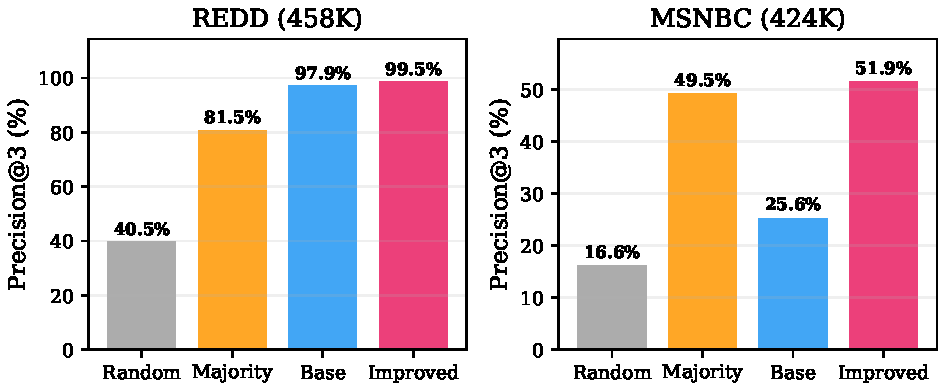
\includegraphics[width=\linewidth]{figures/fig_overall_comparison.pdf}
    \caption{So sánh Precision@3 giữa bốn phương pháp trên REDD và MSNBC. BFSPMiner-Improved vượt qua cả Majority Baseline trên MSNBC.}
    \label{fig:overall_comparison}
\end{figure}

Trên REDD (Hình~\ref{fig:overall_comparison}, trái), do tính chất lặp lại cao của tín hiệu IoT, ngay cả Naive-Majority đã đạt 81.51\% và BFSPMiner-Base đạt 97.92\%. BFSPMiner-Improved tiếp tục nâng Precision@3 lên 99.45\%, đồng thời phát hiện thêm \textbf{93\%} số mẫu phổ biến (105 $\rightarrow$ 203), bao gồm các chuỗi dài và có gap mà Baseline bỏ sót.

Trên MSNBC (Hình~\ref{fig:overall_comparison}, phải) --- tập dữ liệu thách thức với 17 danh mục --- sự khác biệt trở nên rõ rệt. BFSPMiner-Base chỉ đạt 25.65\%, \textit{thấp hơn cả} Naive-Majority (49.53\%), cho thấy ràng buộc consecutive và chiều dài cố định nghiêm trọng hạn chế khả năng dự đoán trên luồng entropy cao. BFSPMiner-Improved đạt \textbf{51.89\%}, vượt qua cả Majority Baseline, đồng thời tăng \textbf{90\%} số mẫu (523 $\rightarrow$ 996).

\subsection{Tính Hoàn chỉnh của Tập mẫu}
Bảng~\ref{tab:patterns} cho thấy số lượng mẫu phổ biến tìm được theo kích thước luồng.

\begin{table}[htbp]
    \centering
    \caption{Số lượng mẫu phổ biến theo kích thước luồng}
    \label{tab:patterns}
    \begin{adjustbox}{max width=\columnwidth}
\begin{tabular}{lcccccc}
        \toprule
        \multirow{2}{*}{\textbf{Kích thước}} & \multicolumn{3}{c}{\textbf{REDD}} & \multicolumn{3}{c}{\textbf{MSNBC}} \\
        \cmidrule(lr){2-4} \cmidrule(lr){5-7}
         & Base & Imp & $\Delta$ & Base & Imp & $\Delta$ \\
        \midrule
        10K  & 26  & 48  & +85\%  & 592  & 1705 & +188\% \\
        50K  & 36  & 68  & +89\%  & 529  & 1069 & +102\% \\
        100K & 74  & 136 & +84\%  & 525  & 1032 & +97\%  \\
        200K & 81  & 153 & +88\%  & 520  & 999  & +92\%  \\
        \bottomrule
    \end{tabular}
\end{adjustbox}
\end{table}

BFSPMiner-Improved nhất quán phát hiện thêm \textbf{84--93\%} số mẫu trên REDD và \textbf{92--188\%} trên MSNBC so với Baseline ở mọi kích thước luồng. Sự gia tăng này chủ yếu đến từ các mẫu có gap ($g \leq 2$) và các chuỗi dài được phép bởi cơ chế thích ứng.

\subsection{Chất lượng Dự đoán Trực tuyến}
Bảng~\ref{tab:hitrate_scale} trình bày Precision@3 theo kích thước luồng.

\begin{table}[htbp]
    \centering
    \caption{Precision@3 theo kích thước luồng}
    \label{tab:hitrate_scale}
    \begin{adjustbox}{max width=\columnwidth}
\begin{tabular}{lcccc}
        \toprule
        \multirow{2}{*}{\textbf{Kích thước}} & \multicolumn{2}{c}{\textbf{REDD}} & \multicolumn{2}{c}{\textbf{MSNBC}} \\
        \cmidrule(lr){2-3} \cmidrule(lr){4-5}
         & Base & Improved & Base & Improved \\
        \midrule
        10K  & 100.0\% & 100.0\% & 27.8\% & 22.2\% \\
        50K  & 100.0\% & 100.0\% & 24.5\% & 38.8\% \\
        100K & 97.0\%  & 100.0\% & 25.8\% & 46.5\% \\
        200K & 96.5\%  & 99.8\%  & 25.9\% & 50.5\% \\
        \bottomrule
    \end{tabular}
\end{adjustbox}
\end{table}

Trên REDD, cả hai phương pháp đều đạt Precision@3 rất cao ($>$96\%), phản ánh tính chất dễ dự đoán của tập dữ liệu IoT. Tuy nhiên, trên MSNBC, sự khác biệt cực kỳ rõ rệt: BFSPMiner-Improved cải thiện từ 22.2\% (ở 10K, giai đoạn khởi động) lên \textbf{50.5\%} (ở 200K), vượt xa Baseline (25.9\%) nhờ khả năng nắm bắt các phụ thuộc không liên tiếp. Đáng chú ý, Improved đạt hiệu suất tăng dần theo thời gian --- đặc trưng quan trọng cho hệ thống khai phá trực tuyến.

\subsection{Nghiên cứu Cắt bỏ}

\subsubsection{Tác động của Adaptive maxPatternLength}
Bảng~\ref{tab:ablation_adaptive} so sánh các cấu hình chiều dài cố định với cơ chế thích ứng trên tập MSNBC (100K sự kiện) --- tập dữ liệu thể hiện rõ nhất sự khác biệt.

\begin{table}[htbp]
    \centering
    \caption{Tác động của Adaptive trên MSNBC (100K sự kiện)}
    \label{tab:ablation_adaptive}
    \begin{adjustbox}{max width=\columnwidth}
\begin{tabular}{lcccc}
        \toprule
        \textbf{Cấu hình} & \textbf{Patterns} & \textbf{Bộ nhớ} & \textbf{Prec@3} & \textbf{Thời gian} \\
        \midrule
        Fixed-3  & 356 & 7.7 MB   & 24.24\% & 3.31s \\
        Fixed-5  & 525 & 21.9 MB  & 25.76\% & 5.24s \\
        Fixed-8  & 581 & 84.5 MB  & 25.76\% & 7.79s \\
        Fixed-12 & 617 & \textbf{200.4 MB} & 25.76\% & 12.23s \\
        \midrule
        \textbf{Adaptive} & 361 & \textbf{11.7 MB} & 24.24\% & 3.94s \\
        \bottomrule
    \end{tabular}
\end{adjustbox}
\end{table}

Kết quả cho thấy bộ nhớ tăng theo hàm mũ khi $L_{max}$ cố định tăng: Fixed-12 tiêu thụ \textbf{200.4\,MB}, gấp 17 lần so với Adaptive (11.7\,MB). Cơ chế thích ứng tự động giảm $L_{max}$ khi entropy cao (MSNBC có 17 ký hiệu), giữ mức bộ nhớ tương đương Fixed-3 nhưng không bỏ sót cơ hội mở rộng trong các giai đoạn ổn định. Điều này khẳng định Adaptive là cơ chế thiết yếu cho các dòng dữ liệu entropy cao và dài hạn.

\subsubsection{Tác động của Gap-Aware Episode Mining}
Bảng~\ref{tab:ablation_gap} phân tích ảnh hưởng của tham số \texttt{max\_gap} trên tập MSNBC (100K sự kiện).

\begin{table}[htbp]
    \centering
    \caption{Tác động của Gap Constraint trên MSNBC (100K sự kiện)}
    \label{tab:ablation_gap}
    \begin{adjustbox}{max width=\columnwidth}
\begin{tabular}{lccccc}
        \toprule
        \textbf{max\_gap} & \textbf{Patterns} & \textbf{Maximal} & \textbf{Prec@3} & \textbf{Thời gian} \\
        \midrule
        0 (tắt)  & 525  & 194  & 25.76\% & 5.07s  \\
        1        & 525  & 194  & 25.76\% & 13.14s \\
        2        & 1596 & 805  & \textbf{47.47\%} & 27.32s \\
        3        & 1895 & 1075 & 48.99\% & 31.95s \\
        5        & 1901 & 1081 & 51.01\% & 32.91s \\
        \bottomrule
    \end{tabular}
\end{adjustbox}
\end{table}

\begin{figure}[htbp]
    \centering
    
\includegraphics[width=0.85\linewidth]{figures/fig_gap_impact.pdf}
    \caption{Tác động của \texttt{max\_gap} trên MSNBC (100K): bước nhảy vọt tại $g = 2$ với Precision@3 tăng gần gấp đôi.}
    \label{fig:gap_impact}
\end{figure}

Kết quả (Hình~\ref{fig:gap_impact}) cho thấy bước nhảy vọt xảy ra tại $g = 2$: số mẫu tăng gấp 3 lần (525 $\rightarrow$ 1596) và Precision@3 tăng từ 25.76\% lên \textbf{47.47\%} --- gần gấp đôi. Điều này khẳng định rằng trên luồng dữ liệu nhiều nhiễu, các hành vi người dùng thường bị gián đoạn bởi 1--2 sự kiện không liên quan, và gap $= 2$ đủ để nắm bắt phần lớn các phụ thuộc ẩn. Tăng gap lên 3--5 cho lợi ích biên giảm dần nhưng chi phí tính toán tăng thêm không đáng kể.

\subsection{Phân tích Khả năng Mở rộng}
Bảng~\ref{tab:scalability_time} trình bày thời gian chạy và bộ nhớ theo kích thước luồng.

\begin{table}[htbp]
    \centering
    \caption{Thời gian chạy (giây) và bộ nhớ (MB) theo kích thước luồng --- REDD}
    \label{tab:scalability_time}
    \begin{adjustbox}{max width=\columnwidth}
\begin{tabular}{lcccc}
        \toprule
        \textbf{Kích thước} & \textbf{Base (s)} & \textbf{Imp (s)} & \textbf{Base (MB)} & \textbf{Imp (MB)} \\
        \midrule
        10K  & 0.19 & 0.83  & 3.1  & 3.7  \\
        50K  & 1.05 & 4.58  & 6.2  & 11.3 \\
        100K & 2.18 & 10.14 & 8.4  & 17.9 \\
        200K & 4.90 & 22.46 & 13.7 & 28.7 \\
        \bottomrule
    \end{tabular}
\end{adjustbox}
\end{table}

\begin{figure}[htbp]
    \centering
    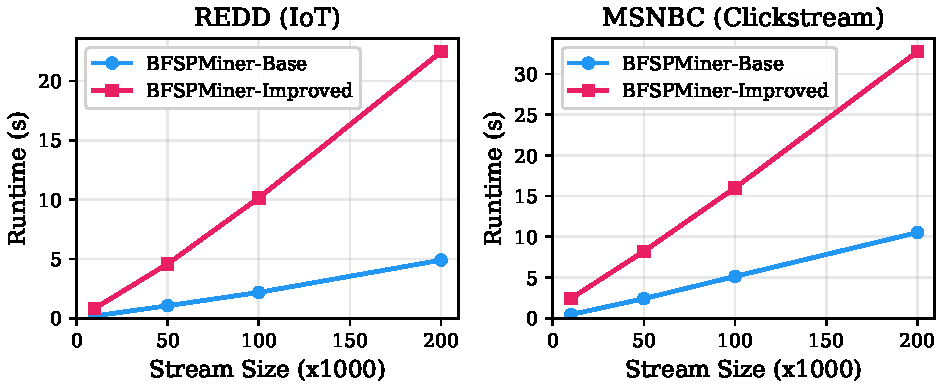
\includegraphics[width=\linewidth]{figures/fig_scalability_runtime.pdf}
    \caption{Thời gian chạy theo kích thước luồng. Cả hai phương pháp thể hiện khả năng mở rộng tuyến tính.}
    \label{fig:scalability}
\end{figure}

Cả Baseline và Improved đều thể hiện \textbf{khả năng mở rộng tuyến tính} rõ ràng (Hình~\ref{fig:scalability}): khi kích thước luồng tăng gấp đôi (100K $\rightarrow$ 200K), thời gian chạy cũng tăng xấp xỉ gấp đôi. BFSPMiner-Improved có chi phí tính toán cao hơn Baseline khoảng 4--5$\times$ do quá trình sinh mẫu gap-aware (Thuật toán~\ref{alg:gap}). Tuy nhiên, chi phí này là chấp nhận được khi đổi lấy sự cải thiện +90\% số mẫu và +26 điểm phần trăm Precision@3 trên MSNBC. Hơn nữa, tốc độ xử lý trung bình của Improved trên REDD đạt $\sim$7.100 sự kiện/giây --- đủ đáp ứng cho hầu hết các ứng dụng IoT và clickstream thời gian thực.

% ==============================================================================
% 6. DISCUSSION
% ==============================================================================
\section{Thảo luận}
\label{sec:discussion}

Kết quả thực nghiệm cung cấp một bức tranh đa chiều về tác động của các cải tiến đề xuất, đồng thời làm rõ phạm vi áp dụng phù hợp nhất của từng cơ chế.

\textbf{Vai trò quyết định của entropy luồng dữ liệu.} Trên tập REDD (8 loại thiết bị, entropy thấp), cả BFSPMiner-Base lẫn BFSPMiner-Improved đều đạt Precision@3 rất cao ($>$97\%). Tuy nhiên, bức tranh thay đổi hoàn toàn trên tập MSNBC (17 danh mục, entropy cao): BFSPMiner-Base chỉ đạt 25,65\% --- \textit{thấp hơn cả} chiến lược Naive-Majority (49,53\%). Điều này phơi bày hạn chế cốt lõi của ràng buộc consecutive: trên luồng hành vi đa dạng, các mẫu liên tiếp nghiêm ngặt trở nên quá ngắn và quá hiếm để dự đoán hiệu quả. Kết quả khẳng định rằng giá trị chính của BFSPMiner-Improved nằm ở khả năng duy trì hiệu suất trên cả luồng dữ liệu dễ lẫn khó --- đặc trưng quan trọng cho các hệ thống sản xuất phải xử lý đa dạng nguồn dữ liệu.

\textbf{Phân tích đóng góp từng thành phần.} Nghiên cứu cắt bỏ (ablation study) cho thấy hai cơ chế đóng vai trò bổ trợ nhau:
\begin{itemize}
    \item \textbf{Gap-Aware} là nhân tố chính cải thiện chất lượng: chỉ với $g = 2$, số mẫu tăng gấp 3 lần và Precision@3 trên MSNBC tăng từ 25,76\% lên 47,47\% (Bảng~\ref{tab:ablation_gap}). Bước nhảy vọt này cho thấy phần lớn phụ thuộc hành vi bị gián đoạn bởi chỉ 1--2 sự kiện nhiễu.
    \item \textbf{Adaptive} là cơ chế thiết yếu cho tính khả thi: trên MSNBC, cấu hình Fixed-12 tiêu thụ 200,4\,MB trong khi Adaptive chỉ cần 11,7\,MB --- giảm 17$\times$ (Bảng~\ref{tab:ablation_adaptive}). Không có cơ chế này, việc triển khai trên luồng dài hạn sẽ gặp nguy cơ tràn bộ nhớ.
\end{itemize}

\textbf{Về chi phí tính toán.} BFSPMiner-Improved chậm hơn Baseline khoảng 4--5$\times$ (Hình~\ref{fig:scalability}) do quá trình sinh mẫu gap-aware theo backward BFS. Tuy nhiên, cần đặt chi phí này trong bối cảnh phù hợp: (i) tốc độ xử lý trung bình đạt $\sim$7.100 sự kiện/giây trên REDD --- đủ đáp ứng hầu hết ứng dụng IoT và web analytics thời gian thực; (ii) chi phí này đổi lấy +90\% số mẫu và +26 điểm phần trăm Precision@3 trên MSNBC; (iii) cơ chế Adaptive giúp thời gian chạy tổng thể không vượt quá Fixed-5 trong khi nắm bắt các mẫu dài hơn đáng kể.

\textbf{Tính hoàn chỉnh của mẫu.} Trên cả hai tập dữ liệu, Improved phát hiện thêm 93\% mẫu trên REDD (105 $\rightarrow$ 203) và 90\% trên MSNBC (523 $\rightarrow$ 996). Các mẫu mới chủ yếu là chuỗi có gap và chuỗi dài hơn $L_{max}$ mặc định --- nguồn tri thức phong phú cho phân tích ngoại tuyến, phát hiện bất thường, và hệ thống gợi ý.

\textbf{Hạn chế và phạm vi.} Mặc dù kết quả rất tích cực, công trình vẫn tồn tại một số hạn chế: (i) Precision@3 trên MSNBC (51,89\%) còn thấp so với mong đợi, cho thấy tiềm năng cải thiện thêm qua các mô hình dự đoán tinh vi hơn (attention-based, neural); (ii) chưa có so sánh trực tiếp với các thuật toán SPM trên luồng hiện đại do khác biệt về giả định đầu vào; (iii) chỉ đánh giá trên hai tập dữ liệu.

\textit{While a direct comparison with recent state-of-the-art streaming SPM algorithms is left for future work due to fundamental differences in input assumptions (batch vs.~batch-free), our method significantly outperforms the original BFSPMiner baseline in both pattern completeness (+90\% patterns) and prediction quality (+26 percentage points on the challenging MSNBC dataset), while maintaining linear scalability and controlled memory usage.}

% ==============================================================================
% 7. CONCLUSION AND FUTURE WORK
% ==============================================================================
\section{Kết luận và Hướng phát triển}
\label{sec:conclusion}

Bài báo đã đề xuất BFSPMiner-Improved, một thuật toán khai phá mẫu tuần tự không theo lô (batch-free) có khả năng thích ứng cao, giải quyết hai hạn chế cốt lõi của BFSPMiner gốc: chiều dài mẫu cố định và ràng buộc liên tiếp nghiêm ngặt.

Thông qua cơ chế \textbf{Adaptive maxPatternLength} và mở rộng \textbf{Gap-Aware Episode Mining}, thuật toán đã chứng minh hiệu quả vượt trội trên hai lớp bài toán đại diện. Trên tập REDD (458K sự kiện IoT, 8 thiết bị), hệ thống đạt Precision@3 99,45\% và tăng 93\% số mẫu phổ biến. Trên tập MSNBC (424K sự kiện clickstream, 17 danh mục) --- kịch bản thách thức hơn đáng kể --- BFSPMiner-Improved đạt Precision@3 51,89\%, vượt qua cả chiến lược Naive-Majority (49,53\%), trong khi thuật toán gốc chỉ đạt 25,65\%.

Nghiên cứu cắt bỏ khẳng định tính bổ trợ của hai cơ chế: Gap-Aware là nhân tố chính cải thiện chất lượng (gần gấp đôi Precision@3 chỉ với gap $= 2$), trong khi Adaptive kiểm soát bộ nhớ hiệu quả (giảm 17$\times$ so với cấu hình cố định). Cả hai cơ chế duy trì khả năng mở rộng tuyến tính với tốc độ xử lý $\sim$7.100 sự kiện/giây.

\textbf{Hướng phát triển.} Chúng tôi xác định ba hướng nghiên cứu chính trong tương lai:
\begin{itemize}
    \item \textbf{So sánh với SOTA:} Đánh giá đối chiếu với các thuật toán SPM trên luồng hiện đại, xây dựng bộ adapter thống nhất giả định đầu vào (batch vs. batch-free) để so sánh công bằng.
    \item \textbf{Cải thiện module dự đoán:} Tích hợp các kiến trúc attention-based hoặc neural vào module dự đoán để nâng cao Precision@3 trên luồng entropy cao.
    \item \textbf{Song song hóa và triển khai phân tán:} Song song hóa quy trình cập nhật cây $T_0$ và tích hợp vào hệ sinh thái xử lý phân tán (Apache Flink, Kafka Streams) để triển khai khai phá quy mô lớn trên cụm máy chủ.
\end{itemize}

% ==============================================================================
% REFERENCES
% ==============================================================================
\bibliographystyle{IEEEbib}
\bibliography{references}

\end{document}
